
	\begin{table}[H]
    \centering
		\begin{tabular}{|c|c|c||c|c|c|}
			\hline
			\rowcolor[rgb]{0.21,0.69,0.87}\multicolumn{6}{|c|}{  \textbf{ {Configuración Pines de entrada}}} \\
			\hline \hline
			\multicolumn{3}{|c|}{  \textbf{ {SensorVoy (4bits)}}} & \multicolumn{3}{|c|}{\textbf{SensorEstoy (4bits)}} \\
			\hline
			SensorVoy[0] & SW0 & F12 & SensorEstoy[0] & BTN0 & M13 \\
			\hline
			SensorVoy[1] & SW1 & G12 & SensorEstoy[1] & BTN1 & M14 \\
			\hline
			SensorVoy[2] & SW2 & H14 & SensorEstoy[2] & BTN2 & L13 \\
			\hline
			SensorVoy[3] & SW3 & H13 & SensorEstoy[3] & BTN3 & L14 \\
			\hline
		\end{tabular}
		\caption{ Configuración de los pines de entrada con las entradas del sistema }
		\label{tab:pinEntradas}
	\end{table}

	\begin{table}[H]
    \centering
		\begin{tabular}{|c|c|}
			\hline
			\rowcolor[rgb]{0.21,0.69,0.87}\multicolumn{2}{|c|}{  \textbf{ {Configuración pin CLK}}} \\
			\hline \hline
			CLK & T9 \\ 
			\hline
		\end{tabular}
		\caption{ Configuración del pin para el CLK }
		\label{tab:pinCLK}
	\end{table}

	\begin{table}[H]
    \centering
		\begin{tabular}{|c|c||c|c|c|}
			\hline
			\rowcolor[rgb]{0.21,0.69,0.87}\multicolumn{4}{|c|}{  \textbf{ {Configuración Pines de los displays de 7 segmentos}}} \\
			\hline \hline
			\multicolumn{2}{|c|}{  \textbf{ { Salida7s (7bits)}}} & \multicolumn{2}{|c|}{\textbf{Ánodos de Control}} \\
			\hline
			Salida7s[0] & E14 & Motor & AN0 & D14 \\
			\hline
			Salida7s[1] & G13 & Puerta & AN1 & G14 \\
			\hline
			Salida7s[2] & N15 & PisoVoy & AN2 & F14 \\
			\hline
			Salida7s[3] & P15 & PisoEstoy & AN3 & E13 \\
			\hline
			Salida7s[4] & R16 & - & - & - \\
			\hline
			Salida7s[5] & F13 & - & - & - \\
			\hline
			Salida7s[6] & N16 & - & - & - \\
			\hline
		\end{tabular}
		\caption{ Configuración de los pines de salida al display de 7 segmentos }
		\label{tab:pin7s}
	\end{table}
	

\subsection{Caso de Uso Práctico:}
	
	Antes de poder hacer una comprobación del funcionamiento de la maqueta debemos conocer sobre que componentes se visualizará la información:
	
	\begin{figure}[H]
        \centering
        \includegraphics[width = 0.6\textwidth ]{CasoUso/0.jpg}
        \caption{Distribución salidas/entradas de la maqueta en la Spartan-3}
        \label{fig:Spartan3Interfaz}
    \end{figure}
    
    
    \begin{itemize}
	    \item 1. Memoria 2: se ve que piso se ha guardado iluminándose el LED de dicha posición (De derecha a izquierda en orden ascendente).
	    \item 2. Memoria 1: Equivalente al anterior, refleja la posición guardada en la memoria 1.
	    \item 3. Emulan los finales de carrera para ver en qué piso se encuentra el ascensor. De derecha a izquierda en orden ascendente de pisos.
	    \item 4. Emulan los botones para seleccionar el piso al que se desea ir. De derecha a izquierda en orden ascendente de pisos.
	    \item 5. Displays para mostrar la información, se puede ver a continuación que se muestra en cada display.
	\end{itemize} 
	
	\begin{figure}[H]
        \centering
        \includegraphics[width = 0.6\textwidth ]{CasoUso/0_1.jpg}
        \caption{Distibución de las salidas a los displays}
        \label{fig:Spartan3InterfazDisplays}
    \end{figure}
    
    \begin{itemize}
		    \item  D1. Piso actual, marcado por los finales de carrera.
		    \item  D2. Piso objetivo, al que quiero ir.
		    \item  D3. Funcionamiento de la puerta.
		    \item  D4. Funcionamiento del motor.
	\end{itemize} 
	

    
	\begin{longtable}{cm{0.2\textwidth}cm{0.2\textwidth}}
	\centering
		 \includegraphics[width = 0.25\textwidth ]{CasoUso/2.jpg} & 1. Al arrancar o resetear el sistema tanto el piso objetivo como el piso actual se inicializan a 0, a la espera de recibir información del sistema real. En este tipo de indeterminaciones el ascensor permanece parado con la puerta abierta. &
		 \includegraphics[width = 0.25\textwidth ]{CasoUso/3.jpg} & 2. Se pasa información sobre los pisos, en este caso el ascensor se situa en el primer piso. Tanto el piso actual como el objetivo son el mismo (1,1), el ascensor permanece parado (-) con la puerta abierta (A).  \\
		 \includegraphics[width = 0.25\textwidth ]{CasoUso/4.jpg} & 3. Se marca el cuarto piso como objetivo, la puerta se cierra (C) y el ascensor comienza a subir (S). & 
		  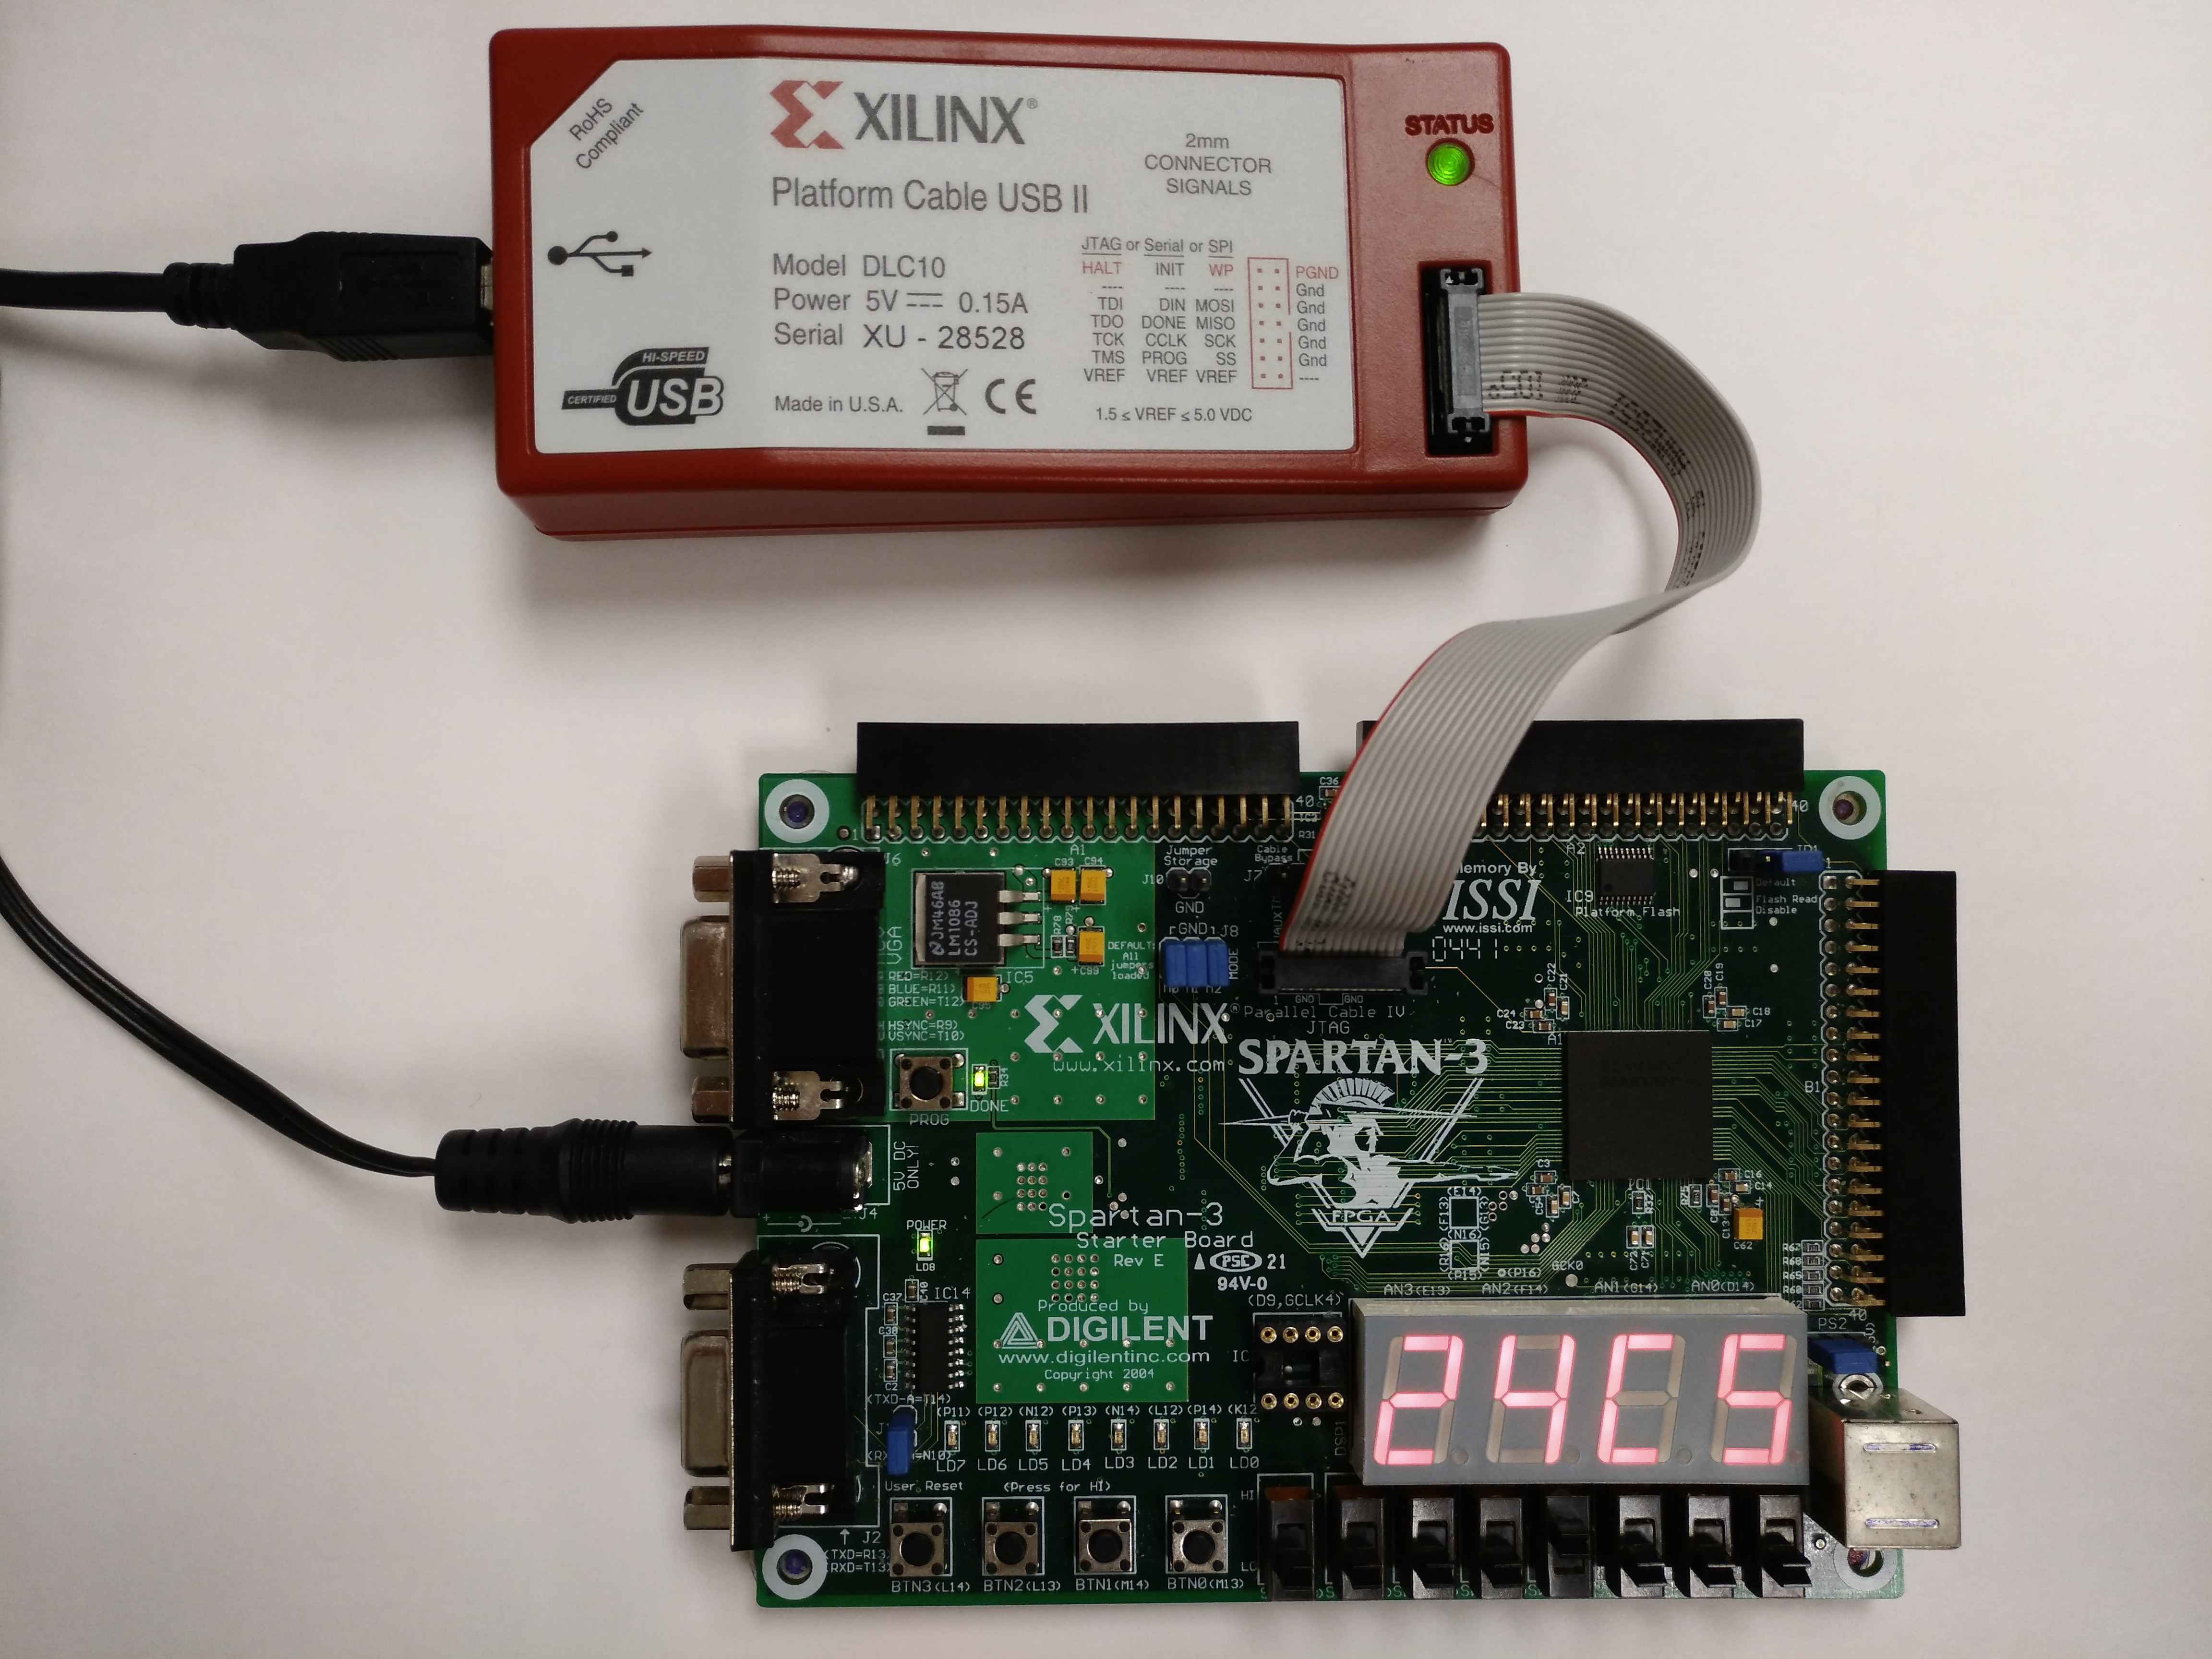
\includegraphics[width = 0.25\textwidth ]{CasoUso/5.jpg} & 4. Según pasa por los pisos intermedios se actualiza el display de piso actual, el ascensor sigue cerrado y subiendo.  \\
		 \includegraphics[width = 0.25\textwidth ]{CasoUso/6.jpg} & 5.  Cuando llega a la planta deseada, el ascensor se detiene y la puerta se abre. & 
		  \includegraphics[width = 0.25\textwidth ]{CasoUso/7.jpg} & 6.  Al marcar un piso inferior, el ascensor se cierra y comienza a descender (B). \\
		 \includegraphics[width = 0.25\textwidth ]{CasoUso/8.jpg} & 7. En este punto podemos marcar otro piso que queda registrado en la memoria. En este caso se marca el tres, que se ve reflejado en el tercer LED de los correspondientes a la memoria 1. & 
		  \includegraphics[width = 0.25\textwidth ]{CasoUso/9.jpg} & 8. Mientras sigue bajando se registra otro piso, el 2 que se guarda en la segunda memoria, viéndose reflejado en el segundo led de los correspondientes a dicha memoria. \\
		 \includegraphics[width = 0.25\textwidth ]{CasoUso/9.1.jpg} & 9. Cuando el ascensor llega al piso objetivo, que era el primero, el ascensor permanece abierto y parado durante un tiempo especificado (para simularlo espera un segundo). & 
		 \includegraphics[width = 0.25\textwidth ]{CasoUso/10.jpg} & 10.  Una vez ha esperado dicho tiempo se carga en la memoria el siguiente dato, el piso tres al cual nos dirigiremos ahora. El guardado en la memoria dos pasa a la primera (que será el siguiente piso), una vez llegado al tercer piso nos dirigimos al segundo. Estos ya no se reflejan en los LEDs destinados a la memoria, si no que vemos que se ha marcado el cuarto piso al que se ha llamado.\\
		  \includegraphics[width = 0.25\textwidth ]{CasoUso/12.jpg} & 10.  Una vez ha llegado al tercer piso nos dirigimos al segundo. Estos ya no se reflejan en los LEDs destinados a la memoria, si no que vemos que se ha marcado el cuarto piso. &
		 \includegraphics[width = 0.25\textwidth ]{CasoUso/13.jpg} & 11. Cuando llega al segundo piso se carga el cuarto y la memoria queda vacia. \\ 
		  \includegraphics[width = 0.25\textwidth ]{CasoUso/14.jpg} & 12. Una vez ha llegado al cuarto piso el ascensor se para y la puerta se abre. & - & - \\
	\end{longtable}